\ifx\wholebook\relax\else
\documentclass{report}
\usepackage{times}
\usepackage{epsfig}
\usepackage{alltt}
\usepackage{xspace}
\usepackage{graphicx}
\usepackage{ifpdf}
\usepackage{ifthen}
\usepackage{amsmath}
\usepackage{a4wide}

\graphicspath{{figures/}} 

\ifpdf
\DeclareGraphicsExtensions{.pdf, .jpg, .tif, .png}
\else
\DeclareGraphicsExtensions{.eps, .jpg}
\fi

\newboolean{toseecomment}
\setboolean{toseecomment}{false}
%%change to false to hidde comment 
\newcommand{\comment}[1]{\ifthenelse{\boolean{toseecomment}}{$\blacktriangleright$ \textit{#1}$\blacktriangleleft$}{}}

\newcommand{\commented}[1]{}

\newboolean{seevwspecific}
\setboolean{seevwspecific}{true}
\newcommand{\vwspecific}[1]{\ifthenelse{\boolean{seevwspecific}}{#1}{}}

\newboolean{seecategoryspecific}
\setboolean{seecategoryspecific}{false}
\newcommand{\categoryspecific}[1]{\ifthenelse{\boolean{seecategoryspecific}}{#1}{}}

\newboolean{seestorespecific}
\setboolean{seestorespecific}{true}
\newcommand{\storespecific}[1]{\ifthenelse{\boolean{seestorespecific}}{#1}{}}

\newboolean{seesqueakspecific}
\setboolean{seesqueakspecific}{false}
\newcommand{\squeakspecific}[1]{\ifthenelse{\boolean{seesqueakspecific}}{#1}{}}


\newcommand{\category}[0]
{\ifthenelse{\boolean{seestorespecific}}
	{package\xspace}
	{category\xspace}}

\newcommand{\ct}[1]{\texttt{#1}\xspace}
\newcommand{\stc}[1]{{\small {\sf #1}}\xspace}
\newcommand{\ST}{{\textsc Smalltalk}\xspace}
\newcommand{\tab}{\makebox[4em]{}}
\newcommand{\ttt}[1]{{\tt #1}}
\newcommand{\chev}{\ttt{>>}}
\newcommand{\vw}{VisualWorks\xspace}
\newcommand{\sq}{Squeak\xspace}
\newcommand{\store}{Store\xspace}
\renewcommand{\chaptername}{Exercise}
\newcommand{\exercise}{\vspace{0.2cm}\noindent \textbf{Exercise:}\xspace}

\newsavebox{\fminibox}
\newlength{\fminilength}

% Fait un truc encadre
\newenvironment{fminipage}[1][\linewidth]
  {\setlength{\fminilength}{#1-2\fboxsep-2\fboxrule}
        \begin{lrbox}{\fminibox}\begin{minipage}{\fminilength}}
  { \end{minipage}\end{lrbox}\noindent\fbox{\usebox{\fminibox}}}

% Pareil mais pas encadre (a utiliser pour ne pas couper une fonction

\newenvironment{nminipage}[1][\linewidth]
  {\setlength{\fminilength}{#1}
        \begin{lrbox}{\fminibox}\begin{minipage}{\fminilength}}
  { \end{minipage}\end{lrbox}\noindent\mbox{\usebox{\fminibox}}}

% Un alltt encadre
\newenvironment{falltt}
  {\vspace*{0.3cm}\begin{fminipage}\begin{alltt}}
  {\end{alltt}\end{fminipage}\vspace*{0.3cm}}

% Un alltt pas encadre
\newenvironment{nalltt}
  {\vspace*{0.3cm}\begin{nminipage}\begin{alltt}}
  {\end{alltt}\end{nminipage}\vspace*{0.3cm}}

% Une fonction encadree
\newenvironment{ffonction}[1]
  {\begin{fonction}[#1]
        \begin{fminipage}
\begin{alltt}
\rule{\linewidth}{0.5pt}}
{\end{alltt}\end{fminipage}\end{fonction}}

\newenvironment{codeonepage}
  {\begin{nminipage}\vspace*{0.2cm}\hrule\vspace*{0.1cm}
\begin{alltt}}
  {\end{alltt} \vspace*{-0.2cm}\hrule \vspace*{0.2cm} \end{nminipage}}

\newenvironment{code}
  {\vspace*{0.1cm}\hrule\vspace*{-0.1cm}\begin{alltt}}
  {\end{alltt}\vspace*{-0.2cm}\hrule \vspace*{0.1cm}}


\begin{document}
\fi

\chapter{Fun with Bots Inc}

\mainauthor{St\'ephane Ducasse}

The goal of this chapter is to get you started with some programming by steering graphical robots. We use the contents of the book Squeak: Learn programming with Robots by St�phane Ducasse, Apress Publishers, 2005 (http://smallwiki.unibe.ch/botsinc/). 

More information on http://www.apress.com/book/bookDisplay.html?bID=444 

\section*{Getting the environment}
Go to http://smallwiki.unibe.ch/botsinc/ and download the distribution for your machine. 
Follow the instructions described page http://smallwiki.unibe.ch/botsinc/installation/ (Unzip it and drap the file name ready.image on the exe file). 

Watch the videos you can find at http://www.iam.unibe.ch/~ducasse/Web/BotsInc/Videos/ and reproduce them during the following exercises.

\section{Create and talking}


Create a robot and talk to it (video 1). You can get the list of action bringing the menu and selecting vocabulary.

\begin{itemize}
\item Draw a square of 200 pixels
\item Draw a rectangle of 100 and 200 pixels
\end{itemize}

\section{Writing Scripts}
Direct interaction does not scale. So we propose you to write scripts as shown in the video 3. 

\begin{itemize}
\item Write a script that draws a square of 200 pixels.
\item Write a script that draws a rectangle of 100 and 200 pixels.
\end{itemize}


\section{Looping}
Read chapter 7 on loop http://smallwiki.unibe.ch/botsinc/chaptersamples/

\begin{itemize}
\item Using a loop write a script that draws a square of 100.
\item Using a loop write a script that draws a rectangle of 100 and 200 pixels.
\item Write a script that draws a stair case (experience 7.7)
\item Try to reproduce Figure 7-11.
\end{itemize}

\section{Variables}
Watch video 5 that introduces the use of variables. There the variable l is incremented
each step of the loop. Redo the experiment shown by the video. Using the same technique, draw a staircase whose step increase regularly. Do not watch at video 6.


\section{Methods: Naming Scripts}
Scripts are powerful but difficult to reuse. First get a code browser (an editor to define method) (video 7, 8 and 9), then read the extra chapter available at http://www.iam.unibe.ch/$\sim$ducasse/Teaching/CoursAnnecy/0506-MDSI/4916\_Ch12\_FINAL.pdf.

Follow the chapter and define the methods asked there and to the exercises.

\section{Composing methods}
Read chapter 13 available http://smallwiki.unibe.ch/botsinc/chaptersamples/ and do the exercises. 

Now using the method square define the following Figures:

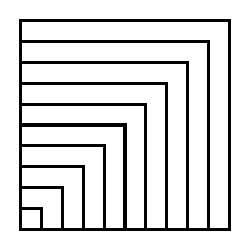
\includegraphics[width=6cm]{Argmirescr}


\includegraphics[width=6cm]{damier}
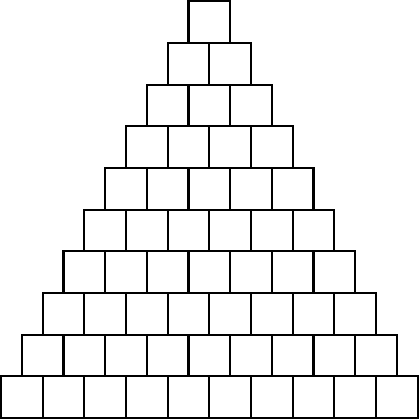
\includegraphics[width=6cm]{cubesandcentpyra}


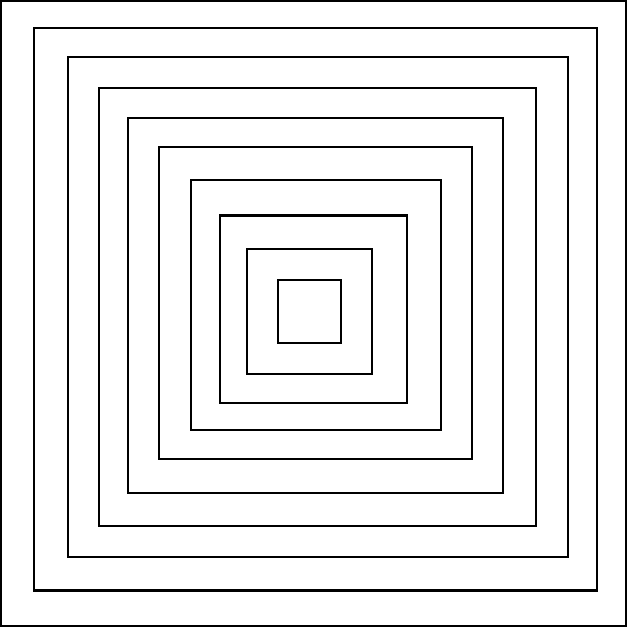
\includegraphics[width=6cm]{corridor}
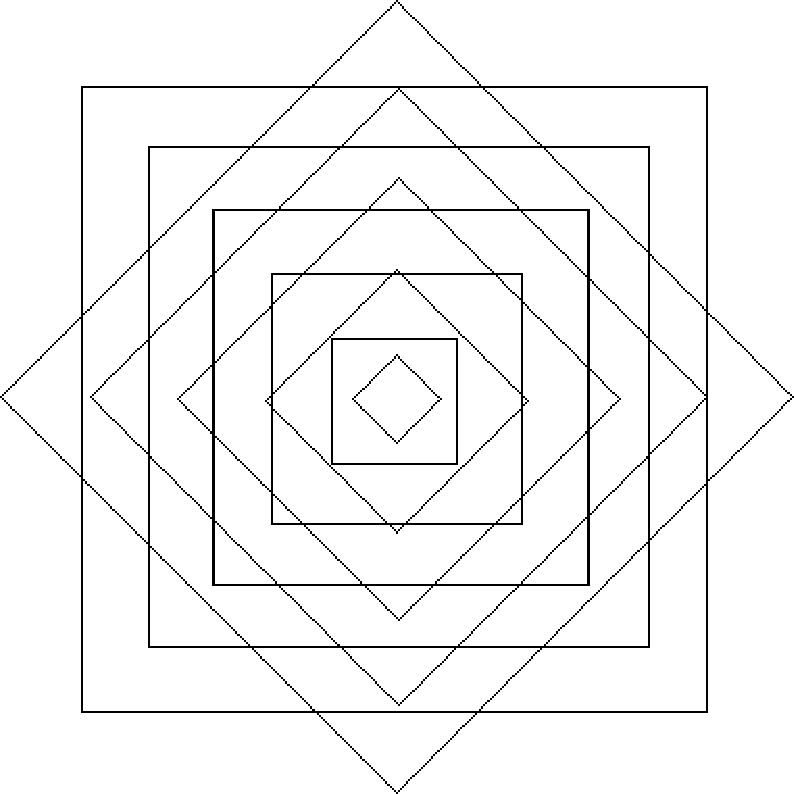
\includegraphics[width=6cm]{mire}

Hints: it may be appropriate to define another method square that draws a square
centered around a point. 

\ifx\wholebook\relax\else\end{document}\fi
